\documentclass[1p]{elsarticle_modified}
%\bibliographystyle{elsarticle-num}

%\usepackage[colorlinks]{hyperref}
%\usepackage{abbrmath_seonhwa} %\Abb, \Ascr, \Acal ,\Abf, \Afrak
\usepackage{amsfonts}
\usepackage{amssymb}
\usepackage{amsmath}
\usepackage{amsthm}
\usepackage{scalefnt}
\usepackage{amsbsy}
\usepackage{kotex}
\usepackage{caption}
\usepackage{subfig}
\usepackage{color}
\usepackage{graphicx}
\usepackage{xcolor} %% white, black, red, green, blue, cyan, magenta, yellow
\usepackage{float}
\usepackage{setspace}
\usepackage{hyperref}

\usepackage{tikz}
\usetikzlibrary{arrows}

\usepackage{multirow}
\usepackage{array} % fixed length table
\usepackage{hhline}

%%%%%%%%%%%%%%%%%%%%%
\makeatletter
\renewcommand*\env@matrix[1][\arraystretch]{%
	\edef\arraystretch{#1}%
	\hskip -\arraycolsep
	\let\@ifnextchar\new@ifnextchar
	\array{*\c@MaxMatrixCols c}}
\makeatother %https://tex.stackexchange.com/questions/14071/how-can-i-increase-the-line-spacing-in-a-matrix
%%%%%%%%%%%%%%%

\usepackage[normalem]{ulem}

\newcommand{\msout}[1]{\ifmmode\text{\sout{\ensuremath{#1}}}\else\sout{#1}\fi}
%SOURCE: \msout is \stkout macro in https://tex.stackexchange.com/questions/20609/strikeout-in-math-mode

\newcommand{\cancel}[1]{
	\ifmmode
	{\color{red}\msout{#1}}
	\else
	{\color{red}\sout{#1}}
	\fi
}

\newcommand{\add}[1]{
	{\color{blue}\uwave{#1}}
}

\newcommand{\replace}[2]{
	\ifmmode
	{\color{red}\msout{#1}}{\color{blue}\uwave{#2}}
	\else
	{\color{red}\sout{#1}}{\color{blue}\uwave{#2}}
	\fi
}

\newcommand{\Sol}{\mathcal{S}} %segment
\newcommand{\D}{D} %diagram
\newcommand{\A}{\mathcal{A}} %arc


%%%%%%%%%%%%%%%%%%%%%%%%%%%%%5 test

\def\sl{\operatorname{\textup{SL}}(2,\Cbb)}
\def\psl{\operatorname{\textup{PSL}}(2,\Cbb)}
\def\quan{\mkern 1mu \triangleright \mkern 1mu}

\theoremstyle{definition}
\newtheorem{thm}{Theorem}[section]
\newtheorem{prop}[thm]{Proposition}
\newtheorem{lem}[thm]{Lemma}
\newtheorem{ques}[thm]{Question}
\newtheorem{cor}[thm]{Corollary}
\newtheorem{defn}[thm]{Definition}
\newtheorem{exam}[thm]{Example}
\newtheorem{rmk}[thm]{Remark}
\newtheorem{alg}[thm]{Algorithm}

\newcommand{\I}{\sqrt{-1}}
\begin{document}

%\begin{frontmatter}
%
%\title{Boundary parabolic representations of knots up to 8 crossings}
%
%%% Group authors per affiliation:
%\author{Yunhi Cho} 
%\address{Department of Mathematics, University of Seoul, Seoul, Korea}
%\ead{yhcho@uos.ac.kr}
%
%
%\author{Seonhwa Kim} %\fnref{s_kim}}
%\address{Center for Geometry and Physics, Institute for Basic Science, Pohang, 37673, Korea}
%\ead{ryeona17@ibs.re.kr}
%
%\author{Hyuk Kim}
%\address{Department of Mathematical Sciences, Seoul National University, Seoul 08826, Korea}
%\ead{hyukkim@snu.ac.kr}
%
%\author{Seokbeom Yoon}
%\address{Department of Mathematical Sciences, Seoul National University, Seoul, 08826,  Korea}
%\ead{sbyoon15@snu.ac.kr}
%
%\begin{abstract}
%We find all boundary parabolic representation of knots up to 8 crossings.
%
%\end{abstract}
%\begin{keyword}
%    \MSC[2010] 57M25 
%\end{keyword}
%
%\end{frontmatter}

%\linenumbers
%\tableofcontents
%
\newcommand\colored[1]{\textcolor{white}{\rule[-0.35ex]{0.8em}{1.4ex}}\kern-0.8em\color{red} #1}%
%\newcommand\colored[1]{\textcolor{white}{ #1}\kern-2.17ex	\textcolor{white}{ #1}\kern-1.81ex	\textcolor{white}{ #1}\kern-2.15ex\color{red}#1	}

{\Large $\underline{12n_{0418}~(K12n_{0418})}$}

\setlength{\tabcolsep}{10pt}
\renewcommand{\arraystretch}{1.6}
\vspace{1cm}\begin{tabular}{m{100pt}>{\centering\arraybackslash}m{274pt}}
\multirow{5}{120pt}{
	\centering
	\includegraphics[width=112pt]{../../../GIT/diagram.site/Diagrams/png/2507_12n_0418.png}\\
\ \ \ A knot diagram\footnotemark}&
\allowdisplaybreaks
\textbf{Linearized knot diagam} \\
\cline{2-2}
 &
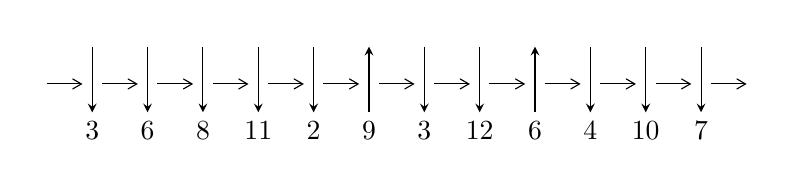
\begin{tikzpicture}[x=20pt, y=17pt]
	% nodes
	\node (C0) at (0, 0) {};
	\node (C1) at (1, 0) {};
	\node (C1U) at (1, +1) {};
	\node (C1D) at (1, -1) {3};

	\node (C2) at (2, 0) {};
	\node (C2U) at (2, +1) {};
	\node (C2D) at (2, -1) {6};

	\node (C3) at (3, 0) {};
	\node (C3U) at (3, +1) {};
	\node (C3D) at (3, -1) {8};

	\node (C4) at (4, 0) {};
	\node (C4U) at (4, +1) {};
	\node (C4D) at (4, -1) {11};

	\node (C5) at (5, 0) {};
	\node (C5U) at (5, +1) {};
	\node (C5D) at (5, -1) {2};

	\node (C6) at (6, 0) {};
	\node (C6U) at (6, +1) {};
	\node (C6D) at (6, -1) {9};

	\node (C7) at (7, 0) {};
	\node (C7U) at (7, +1) {};
	\node (C7D) at (7, -1) {3};

	\node (C8) at (8, 0) {};
	\node (C8U) at (8, +1) {};
	\node (C8D) at (8, -1) {12};

	\node (C9) at (9, 0) {};
	\node (C9U) at (9, +1) {};
	\node (C9D) at (9, -1) {6};

	\node (C10) at (10, 0) {};
	\node (C10U) at (10, +1) {};
	\node (C10D) at (10, -1) {4};

	\node (C11) at (11, 0) {};
	\node (C11U) at (11, +1) {};
	\node (C11D) at (11, -1) {10};

	\node (C12) at (12, 0) {};
	\node (C12U) at (12, +1) {};
	\node (C12D) at (12, -1) {7};
	\node (C13) at (13, 0) {};

	% arrows
	\draw[->,>={angle 60}]
	(C0) edge (C1) (C1) edge (C2) (C2) edge (C3) (C3) edge (C4) (C4) edge (C5) (C5) edge (C6) (C6) edge (C7) (C7) edge (C8) (C8) edge (C9) (C9) edge (C10) (C10) edge (C11) (C11) edge (C12) (C12) edge (C13) ;	\draw[->,>=stealth]
	(C1U) edge (C1D) (C2U) edge (C2D) (C3U) edge (C3D) (C4U) edge (C4D) (C5U) edge (C5D) (C6D) edge (C6U) (C7U) edge (C7D) (C8U) edge (C8D) (C9D) edge (C9U) (C10U) edge (C10D) (C11U) edge (C11D) (C12U) edge (C12D) ;
	\end{tikzpicture} \\
\hhline{~~} \\& 
\textbf{Solving Sequence} \\ \cline{2-2} 
 &
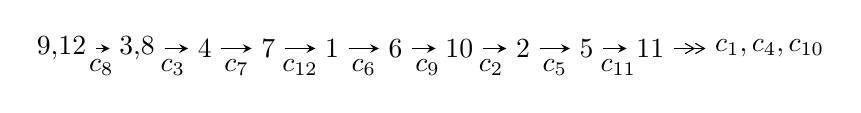
\begin{tikzpicture}[x=23pt, y=7pt]
	% node
	\node (A0) at (-1/8, 0) {9,12};
	\node (A1) at (17/16, 0) {3,8};
	\node (A2) at (17/8, 0) {4};
	\node (A3) at (25/8, 0) {7};
	\node (A4) at (33/8, 0) {1};
	\node (A5) at (41/8, 0) {6};
	\node (A6) at (49/8, 0) {10};
	\node (A7) at (57/8, 0) {2};
	\node (A8) at (65/8, 0) {5};
	\node (A9) at (73/8, 0) {11};
	\node (C1) at (1/2, -1) {$c_{8}$};
	\node (C2) at (13/8, -1) {$c_{3}$};
	\node (C3) at (21/8, -1) {$c_{7}$};
	\node (C4) at (29/8, -1) {$c_{12}$};
	\node (C5) at (37/8, -1) {$c_{6}$};
	\node (C6) at (45/8, -1) {$c_{9}$};
	\node (C7) at (53/8, -1) {$c_{2}$};
	\node (C8) at (61/8, -1) {$c_{5}$};
	\node (C9) at (69/8, -1) {$c_{11}$};
	\node (A10) at (11, 0) {$c_{1},c_{4},c_{10}$};

	% edge
	\draw[->,>=stealth]	
	(A0) edge (A1) (A1) edge (A2) (A2) edge (A3) (A3) edge (A4) (A4) edge (A5) (A5) edge (A6) (A6) edge (A7) (A7) edge (A8) (A8) edge (A9) ;
	\draw[->>,>={angle 60}]	
	(A9) edge (A10);
\end{tikzpicture} \\ 

\end{tabular} \\

\footnotetext{
The image of knot diagram is generated by the software ``\textbf{Draw programme}" developed by Andrew Bartholomew(\url{http://www.layer8.co.uk/maths/draw/index.htm\#Running-draw}), where we modified some parts for our purpose(\url{https://github.com/CATsTAILs/LinksPainter}).
}\phantom \\ \newline 
\centering \textbf{Ideals for irreducible components\footnotemark of $X_{\text{par}}$} 
 
\begin{align*}
I^u_{1}&=\langle 
-3.26934\times10^{56} u^{30}-1.00911\times10^{57} u^{29}+\cdots+1.14470\times10^{59} b-5.53521\times10^{58},\\
\phantom{I^u_{1}}&\phantom{= \langle  }-1.15992\times10^{59} u^{30}-2.78534\times10^{59} u^{29}+\cdots+6.06690\times10^{60} a+1.84407\times10^{61},\\
\phantom{I^u_{1}}&\phantom{= \langle  }u^{31}+2 u^{30}+\cdots-374 u+53\rangle \\
I^u_{2}&=\langle 
2288080379940 u^{21}-13342880074590 u^{20}+\cdots+13036173440749 b+28488698280106,\\
\phantom{I^u_{2}}&\phantom{= \langle  }144701135614458 u^{21}-482252040257618 u^{20}+\cdots+91253214085243 a-23683083359794,\\
\phantom{I^u_{2}}&\phantom{= \langle  }u^{22}-3 u^{21}+\cdots- u-1\rangle \\
\\
\end{align*}
\raggedright * 2 irreducible components of $\dim_{\mathbb{C}}=0$, with total 53 representations.\\
\footnotetext{All coefficients of polynomials are rational numbers. But the coefficients are sometimes approximated in decimal forms when there is not enough margin.}
\newpage
\renewcommand{\arraystretch}{1}
\centering \section*{I. $I^u_{1}= \langle -3.27\times10^{56} u^{30}-1.01\times10^{57} u^{29}+\cdots+1.14\times10^{59} b-5.54\times10^{58},\;-1.16\times10^{59} u^{30}-2.79\times10^{59} u^{29}+\cdots+6.07\times10^{60} a+1.84\times10^{61},\;u^{31}+2 u^{30}+\cdots-374 u+53 \rangle$}
\flushleft \textbf{(i) Arc colorings}\\
\begin{tabular}{m{7pt} m{180pt} m{7pt} m{180pt} }
\flushright $a_{9}=$&$\begin{pmatrix}1\\0\end{pmatrix}$ \\
\flushright $a_{12}=$&$\begin{pmatrix}0\\u\end{pmatrix}$ \\
\flushright $a_{3}=$&$\begin{pmatrix}0.0191188 u^{30}+0.0459104 u^{29}+\cdots+8.09643 u-3.03956\\0.00285607 u^{30}+0.00881553 u^{29}+\cdots+0.315937 u+0.483552\end{pmatrix}$ \\
\flushright $a_{8}=$&$\begin{pmatrix}1\\- u^2\end{pmatrix}$ \\
\flushright $a_{4}=$&$\begin{pmatrix}0.0114818 u^{30}+0.0242158 u^{29}+\cdots+5.92417 u-3.11645\\0.00728253 u^{30}+0.0208089 u^{29}+\cdots+2.31246 u+0.143262\end{pmatrix}$ \\
\flushright $a_{7}=$&$\begin{pmatrix}-0.0125194 u^{30}-0.0332989 u^{29}+\cdots-3.31812 u+2.11184\\0.00904266 u^{30}+0.0208537 u^{29}+\cdots+6.07142 u-1.31372\end{pmatrix}$ \\
\flushright $a_{1}=$&$\begin{pmatrix}-0.0137586 u^{30}-0.0382466 u^{29}+\cdots-5.78489 u+0.627589\\0.00498751 u^{30}+0.0153717 u^{29}+\cdots-0.409851 u+0.438957\end{pmatrix}$ \\
\flushright $a_{6}=$&$\begin{pmatrix}-0.0215620 u^{30}-0.0541526 u^{29}+\cdots-9.38954 u+3.42557\\0.00904266 u^{30}+0.0208537 u^{29}+\cdots+6.07142 u-1.31372\end{pmatrix}$ \\
\flushright $a_{10}=$&$\begin{pmatrix}0.00710160 u^{30}+0.0223768 u^{29}+\cdots+3.65065 u+0.846020\\-0.0153838 u^{30}-0.0339537 u^{29}+\cdots-10.1652 u+1.84167\end{pmatrix}$ \\
\flushright $a_{2}=$&$\begin{pmatrix}-0.00233531 u^{30}-0.00869416 u^{29}+\cdots-2.45300 u-0.381174\\-0.00433511 u^{30}-0.0145092 u^{29}+\cdots-1.18936 u+0.450278\end{pmatrix}$ \\
\flushright $a_{5}=$&$\begin{pmatrix}-0.0154553 u^{30}-0.0361401 u^{29}+\cdots-9.80384 u+3.74041\\0.0228960 u^{30}+0.0534719 u^{29}+\cdots+12.3145 u-2.52457\end{pmatrix}$ \\
\flushright $a_{11}=$&$\begin{pmatrix}0.0170559 u^{30}+0.0494259 u^{29}+\cdots+8.44345 u-0.917949\\-0.0254517 u^{30}-0.0597883 u^{29}+\cdots-13.3489 u+2.51042\end{pmatrix}$\\&\end{tabular}
\flushleft \textbf{(ii) Obstruction class $= -1$}\\~\\
\flushleft \textbf{(iii) Cusp Shapes $= -0.0281078 u^{30}-0.0792191 u^{29}+\cdots-6.22632 u-13.3726$}\\~\\
\newpage\renewcommand{\arraystretch}{1}
\flushleft \textbf{(iv) u-Polynomials at the component}\newline \\
\begin{tabular}{m{50pt}|m{274pt}}
Crossings & \hspace{64pt}u-Polynomials at each crossing \\
\hline $$\begin{aligned}c_{1}\end{aligned}$$&$\begin{aligned}
&u^{31}+59 u^{30}+\cdots-484409 u+120409
\end{aligned}$\\
\hline $$\begin{aligned}c_{2},c_{5}\end{aligned}$$&$\begin{aligned}
&u^{31}+3 u^{30}+\cdots+599 u+347
\end{aligned}$\\
\hline $$\begin{aligned}c_{3},c_{7}\end{aligned}$$&$\begin{aligned}
&u^{31}- u^{30}+\cdots-221 u+527
\end{aligned}$\\
\hline $$\begin{aligned}c_{4},c_{10}\end{aligned}$$&$\begin{aligned}
&u^{31}- u^{30}+\cdots+5 u+13
\end{aligned}$\\
\hline $$\begin{aligned}c_{6},c_{9}\end{aligned}$$&$\begin{aligned}
&u^{31}+2 u^{30}+\cdots+75 u^2-1
\end{aligned}$\\
\hline $$\begin{aligned}c_{8}\end{aligned}$$&$\begin{aligned}
&u^{31}-2 u^{30}+\cdots-374 u-53
\end{aligned}$\\
\hline $$\begin{aligned}c_{11}\end{aligned}$$&$\begin{aligned}
&u^{31}+29 u^{30}+\cdots+2911 u+169
\end{aligned}$\\
\hline $$\begin{aligned}c_{12}\end{aligned}$$&$\begin{aligned}
&u^{31}+2 u^{30}+\cdots-185350 u-50425
\end{aligned}$\\
\hline
\end{tabular}\\~\\
\newpage\renewcommand{\arraystretch}{1}
\flushleft \textbf{(v) Riley Polynomials at the component}\newline \\
\begin{tabular}{m{50pt}|m{274pt}}
Crossings & \hspace{64pt}Riley Polynomials at each crossing \\
\hline $$\begin{aligned}c_{1}\end{aligned}$$&$\begin{aligned}
&y^{31}-183 y^{30}+\cdots+2147685948663 y-14498327281
\end{aligned}$\\
\hline $$\begin{aligned}c_{2},c_{5}\end{aligned}$$&$\begin{aligned}
&y^{31}-59 y^{30}+\cdots-484409 y-120409
\end{aligned}$\\
\hline $$\begin{aligned}c_{3},c_{7}\end{aligned}$$&$\begin{aligned}
&y^{31}-57 y^{30}+\cdots+1881747 y-277729
\end{aligned}$\\
\hline $$\begin{aligned}c_{4},c_{10}\end{aligned}$$&$\begin{aligned}
&y^{31}-29 y^{30}+\cdots+2911 y-169
\end{aligned}$\\
\hline $$\begin{aligned}c_{6},c_{9}\end{aligned}$$&$\begin{aligned}
&y^{31}+34 y^{30}+\cdots+150 y-1
\end{aligned}$\\
\hline $$\begin{aligned}c_{8}\end{aligned}$$&$\begin{aligned}
&y^{31}-10 y^{30}+\cdots+84014 y-2809
\end{aligned}$\\
\hline $$\begin{aligned}c_{11}\end{aligned}$$&$\begin{aligned}
&y^{31}-41 y^{30}+\cdots+4210051 y-28561
\end{aligned}$\\
\hline $$\begin{aligned}c_{12}\end{aligned}$$&$\begin{aligned}
&y^{31}-78 y^{30}+\cdots+44563768850 y-2542680625
\end{aligned}$\\
\hline
\end{tabular}\\~\\
\newpage\flushleft \textbf{(vi) Complex Volumes and Cusp Shapes}
$$\begin{array}{c|c|c}  
\text{Solutions to }I^u_{1}& \I (\text{vol} + \sqrt{-1}CS) & \text{Cusp shape}\\
 \hline 
\begin{aligned}
u &= \phantom{-}0.703721 + 0.744561 I \\
a &= -0.131219 - 0.230843 I \\
b &= -0.150516 + 0.640112 I\end{aligned}
 & -0.71734 - 2.07224 I & -3.68384 + 1.56459 I \\ \hline\begin{aligned}
u &= \phantom{-}0.703721 - 0.744561 I \\
a &= -0.131219 + 0.230843 I \\
b &= -0.150516 - 0.640112 I\end{aligned}
 & -0.71734 + 2.07224 I & -3.68384 - 1.56459 I \\ \hline\begin{aligned}
u &= -0.695433 + 0.780531 I \\
a &= \phantom{-}0.508339 - 0.670000 I \\
b &= \phantom{-}0.329548 + 0.630508 I\end{aligned}
 & -3.81425 + 5.79719 I & -8.30177 - 4.14014 I \\ \hline\begin{aligned}
u &= -0.695433 - 0.780531 I \\
a &= \phantom{-}0.508339 + 0.670000 I \\
b &= \phantom{-}0.329548 - 0.630508 I\end{aligned}
 & -3.81425 - 5.79719 I & -8.30177 + 4.14014 I \\ \hline\begin{aligned}
u &= -0.884098 + 0.327223 I \\
a &= \phantom{-}2.72119 - 0.44116 I \\
b &= -0.58571 + 1.64877 I\end{aligned}
 & -9.20202 + 4.10011 I & -18.4887 - 4.6238 I \\ \hline\begin{aligned}
u &= -0.884098 - 0.327223 I \\
a &= \phantom{-}2.72119 + 0.44116 I \\
b &= -0.58571 - 1.64877 I\end{aligned}
 & -9.20202 - 4.10011 I & -18.4887 + 4.6238 I \\ \hline\begin{aligned}
u &= \phantom{-}1.13855\phantom{ +0.000000I} \\
a &= -1.34619\phantom{ +0.000000I} \\
b &= \phantom{-}0.551542\phantom{ +0.000000I}\end{aligned}
 & -5.55158\phantom{ +0.000000I} & -15.9810\phantom{ +0.000000I} \\ \hline\begin{aligned}
u &= \phantom{-}0.228324 + 0.824059 I \\
a &= -0.020823 - 0.480166 I \\
b &= -0.201885 + 0.199719 I\end{aligned}
 & \phantom{-}1.16898 - 1.90810 I & -3.82691 + 6.03216 I \\ \hline\begin{aligned}
u &= \phantom{-}0.228324 - 0.824059 I \\
a &= -0.020823 + 0.480166 I \\
b &= -0.201885 - 0.199719 I\end{aligned}
 & \phantom{-}1.16898 + 1.90810 I & -3.82691 - 6.03216 I \\ \hline\begin{aligned}
u &= -1.14547\phantom{ +0.000000I} \\
a &= -1.67126\phantom{ +0.000000I} \\
b &= \phantom{-}0.294014\phantom{ +0.000000I}\end{aligned}
 & -10.8570\phantom{ +0.000000I} & -1.07250\phantom{ +0.000000I}\\
 \hline 
 \end{array}$$\newpage$$\begin{array}{c|c|c}  
\text{Solutions to }I^u_{1}& \I (\text{vol} + \sqrt{-1}CS) & \text{Cusp shape}\\
 \hline 
\begin{aligned}
u &= -0.052704 + 0.830178 I \\
a &= \phantom{-}0.688824 + 1.106930 I \\
b &= \phantom{-}1.032010 + 0.511602 I\end{aligned}
 & -0.254185 + 0.523436 I & -8.37978 - 3.05773 I \\ \hline\begin{aligned}
u &= -0.052704 - 0.830178 I \\
a &= \phantom{-}0.688824 - 1.106930 I \\
b &= \phantom{-}1.032010 - 0.511602 I\end{aligned}
 & -0.254185 - 0.523436 I & -8.37978 + 3.05773 I \\ \hline\begin{aligned}
u &= \phantom{-}0.821890\phantom{ +0.000000I} \\
a &= \phantom{-}3.31155\phantom{ +0.000000I} \\
b &= -0.588551\phantom{ +0.000000I}\end{aligned}
 & -15.0143\phantom{ +0.000000I} & -24.8400\phantom{ +0.000000I} \\ \hline\begin{aligned}
u &= -1.093710 + 0.585354 I \\
a &= -0.529184 - 0.132666 I \\
b &= -0.021101 + 0.605842 I\end{aligned}
 & -5.53724 - 1.04949 I & -12.01248 + 0.06352 I \\ \hline\begin{aligned}
u &= -1.093710 - 0.585354 I \\
a &= -0.529184 + 0.132666 I \\
b &= -0.021101 - 0.605842 I\end{aligned}
 & -5.53724 + 1.04949 I & -12.01248 - 0.06352 I \\ \hline\begin{aligned}
u &= \phantom{-}1.296560 + 0.420401 I \\
a &= -1.209060 - 0.052495 I \\
b &= \phantom{-}0.37149 + 1.70399 I\end{aligned}
 & -4.79226 - 2.17270 I & -10.74429 + 3.28820 I \\ \hline\begin{aligned}
u &= \phantom{-}1.296560 - 0.420401 I \\
a &= -1.209060 + 0.052495 I \\
b &= \phantom{-}0.37149 - 1.70399 I\end{aligned}
 & -4.79226 + 2.17270 I & -10.74429 - 3.28820 I \\ \hline\begin{aligned}
u &= \phantom{-}0.525205 + 1.267060 I \\
a &= -0.621188 + 0.802341 I \\
b &= -0.75793 + 1.60948 I\end{aligned}
 & -1.26769 - 5.50031 I & -6.94404 + 6.71659 I \\ \hline\begin{aligned}
u &= \phantom{-}0.525205 - 1.267060 I \\
a &= -0.621188 - 0.802341 I \\
b &= -0.75793 - 1.60948 I\end{aligned}
 & -1.26769 + 5.50031 I & -6.94404 - 6.71659 I \\ \hline\begin{aligned}
u &= \phantom{-}0.526743 + 0.289192 I \\
a &= \phantom{-}0.458089 - 0.578413 I \\
b &= -0.03750 - 1.47275 I\end{aligned}
 & \phantom{-}2.32560 + 0.63901 I & -14.5403 + 2.2459 I\\
 \hline 
 \end{array}$$\newpage$$\begin{array}{c|c|c}  
\text{Solutions to }I^u_{1}& \I (\text{vol} + \sqrt{-1}CS) & \text{Cusp shape}\\
 \hline 
\begin{aligned}
u &= \phantom{-}0.526743 - 0.289192 I \\
a &= \phantom{-}0.458089 + 0.578413 I \\
b &= -0.03750 + 1.47275 I\end{aligned}
 & \phantom{-}2.32560 - 0.63901 I & -14.5403 - 2.2459 I \\ \hline\begin{aligned}
u &= \phantom{-}1.61851\phantom{ +0.000000I} \\
a &= \phantom{-}1.15913\phantom{ +0.000000I} \\
b &= \phantom{-}0.0859312\phantom{ +0.000000I}\end{aligned}
 & -18.4664\phantom{ +0.000000I} & -13.9210\phantom{ +0.000000I} \\ \hline\begin{aligned}
u &= -1.63750 + 0.39106 I \\
a &= \phantom{-}0.729477 + 0.317725 I \\
b &= \phantom{-}0.06541 + 1.72456 I\end{aligned}
 & -12.19770 - 0.58193 I & -13.84300 + 0.10785 I \\ \hline\begin{aligned}
u &= -1.63750 - 0.39106 I \\
a &= \phantom{-}0.729477 - 0.317725 I \\
b &= \phantom{-}0.06541 - 1.72456 I\end{aligned}
 & -12.19770 + 0.58193 I & -13.84300 - 0.10785 I \\ \hline\begin{aligned}
u &= \phantom{-}0.196127\phantom{ +0.000000I} \\
a &= -1.56428\phantom{ +0.000000I} \\
b &= \phantom{-}0.421923\phantom{ +0.000000I}\end{aligned}
 & -0.703748\phantom{ +0.000000I} & -14.3840\phantom{ +0.000000I} \\ \hline\begin{aligned}
u &= -1.36626 + 1.27176 I \\
a &= -0.916122 - 0.700221 I \\
b &= \phantom{-}0.39264 - 2.22764 I\end{aligned}
 & \phantom{-}15.5087 + 12.5998 I & -12.34182 - 4.74713 I \\ \hline\begin{aligned}
u &= -1.36626 - 1.27176 I \\
a &= -0.916122 + 0.700221 I \\
b &= \phantom{-}0.39264 + 2.22764 I\end{aligned}
 & \phantom{-}15.5087 - 12.5998 I & -12.34182 + 4.74713 I \\ \hline\begin{aligned}
u &= -1.23394 + 1.55331 I \\
a &= -0.498680 - 0.733814 I \\
b &= -0.09233 - 2.40682 I\end{aligned}
 & \phantom{-}16.2047 - 2.4749 I & -8.00000 + 0. I\phantom{ +0.000000I} \\ \hline\begin{aligned}
u &= -1.23394 - 1.55331 I \\
a &= -0.498680 + 0.733814 I \\
b &= -0.09233 + 2.40682 I\end{aligned}
 & \phantom{-}16.2047 + 2.4749 I & -8.00000 + 0. I\phantom{ +0.000000I} \\ \hline\begin{aligned}
u &= \phantom{-}1.36828 + 1.45922 I \\
a &= \phantom{-}0.696632 - 0.707290 I \\
b &= -0.22656 - 2.42636 I\end{aligned}
 & -19.0095 - 5.2807 I & -8.00000 + 0. I\phantom{ +0.000000I}\\
 \hline 
 \end{array}$$\newpage$$\begin{array}{c|c|c}  
\text{Solutions to }I^u_{1}& \I (\text{vol} + \sqrt{-1}CS) & \text{Cusp shape}\\
 \hline 
\begin{aligned}
u &= \phantom{-}1.36828 - 1.45922 I \\
a &= \phantom{-}0.696632 + 0.707290 I \\
b &= -0.22656 + 2.42636 I\end{aligned}
 & -19.0095 + 5.2807 I & -8.00000 + 0. I\phantom{ +0.000000I}\\
 \hline 
 \end{array}$$\newpage\newpage\renewcommand{\arraystretch}{1}
\centering \section*{II. $I^u_{2}= \langle 2.29\times10^{12} u^{21}-1.33\times10^{13} u^{20}+\cdots+1.30\times10^{13} b+2.85\times10^{13},\;1.45\times10^{14} u^{21}-4.82\times10^{14} u^{20}+\cdots+9.13\times10^{13} a-2.37\times10^{13},\;u^{22}-3 u^{21}+\cdots- u-1 \rangle$}
\flushleft \textbf{(i) Arc colorings}\\
\begin{tabular}{m{7pt} m{180pt} m{7pt} m{180pt} }
\flushright $a_{9}=$&$\begin{pmatrix}1\\0\end{pmatrix}$ \\
\flushright $a_{12}=$&$\begin{pmatrix}0\\u\end{pmatrix}$ \\
\flushright $a_{3}=$&$\begin{pmatrix}-1.58571 u^{21}+5.28477 u^{20}+\cdots+8.79506 u+0.259531\\-0.175518 u^{21}+1.02353 u^{20}+\cdots-0.370583 u-2.18536\end{pmatrix}$ \\
\flushright $a_{8}=$&$\begin{pmatrix}1\\- u^2\end{pmatrix}$ \\
\flushright $a_{4}=$&$\begin{pmatrix}-1.68041 u^{21}+5.28816 u^{20}+\cdots+10.2237 u+1.91725\\-0.144177 u^{21}+0.875198 u^{20}+\cdots+0.00484553 u-1.90463\end{pmatrix}$ \\
\flushright $a_{7}=$&$\begin{pmatrix}-0.897790 u^{21}+2.29354 u^{20}+\cdots+6.23833 u+4.35533\\0.179274 u^{21}-0.310068 u^{20}+\cdots+0.773322 u+0.158689\end{pmatrix}$ \\
\flushright $a_{1}=$&$\begin{pmatrix}0.481602 u^{21}-2.58266 u^{20}+\cdots-12.9500 u+8.90752\\-0.841311 u^{21}+2.70321 u^{20}+\cdots+1.56148 u+1.61463\end{pmatrix}$ \\
\flushright $a_{6}=$&$\begin{pmatrix}-1.07706 u^{21}+2.60361 u^{20}+\cdots+5.46501 u+4.19664\\0.179274 u^{21}-0.310068 u^{20}+\cdots+0.773322 u+0.158689\end{pmatrix}$ \\
\flushright $a_{10}=$&$\begin{pmatrix}2.71177 u^{21}-8.48610 u^{20}+\cdots-15.1040 u-1.10776\\-1.09714 u^{21}+2.80089 u^{20}+\cdots+2.25750 u+1.05460\end{pmatrix}$ \\
\flushright $a_{2}=$&$\begin{pmatrix}-4.45944 u^{21}+13.6659 u^{20}+\cdots+16.9373 u+6.28405\\-1.17552 u^{21}+4.02353 u^{20}+\cdots+7.62942 u-1.18536\end{pmatrix}$ \\
\flushright $a_{5}=$&$\begin{pmatrix}5.31330 u^{21}-16.8601 u^{20}+\cdots-26.6004 u-4.64301\\1.65088 u^{21}-5.79168 u^{20}+\cdots-8.47517 u+4.32508\end{pmatrix}$ \\
\flushright $a_{11}=$&$\begin{pmatrix}6.16288 u^{21}-19.4046 u^{20}+\cdots-29.4931 u-3.47305\\-0.447926 u^{21}+0.664587 u^{20}+\cdots-3.13848 u+1.76637\end{pmatrix}$\\&\end{tabular}
\flushleft \textbf{(ii) Obstruction class $= 1$}\\~\\
\flushleft \textbf{(iii) Cusp Shapes $= \frac{358582400273224}{91253214085243} u^{21}-\frac{1126227269963647}{91253214085243} u^{20}+\cdots-\frac{215672464858020}{91253214085243} u-\frac{410928767453229}{91253214085243}$}\\~\\
\newpage\renewcommand{\arraystretch}{1}
\flushleft \textbf{(iv) u-Polynomials at the component}\newline \\
\begin{tabular}{m{50pt}|m{274pt}}
Crossings & \hspace{64pt}u-Polynomials at each crossing \\
\hline $$\begin{aligned}c_{1}\end{aligned}$$&$\begin{aligned}
&u^{22}-18 u^{21}+\cdots-10 u+1
\end{aligned}$\\
\hline $$\begin{aligned}c_{2}\end{aligned}$$&$\begin{aligned}
&u^{22}+2 u^{21}+\cdots-2 u-1
\end{aligned}$\\
\hline $$\begin{aligned}c_{3}\end{aligned}$$&$\begin{aligned}
&u^{22}-10 u^{20}+\cdots+4 u-1
\end{aligned}$\\
\hline $$\begin{aligned}c_{4}\end{aligned}$$&$\begin{aligned}
&u^{22}-8 u^{20}+\cdots+2 u+1
\end{aligned}$\\
\hline $$\begin{aligned}c_{5}\end{aligned}$$&$\begin{aligned}
&u^{22}-2 u^{21}+\cdots+2 u-1
\end{aligned}$\\
\hline $$\begin{aligned}c_{6}\end{aligned}$$&$\begin{aligned}
&u^{22}+3 u^{21}+\cdots- u+1
\end{aligned}$\\
\hline $$\begin{aligned}c_{7}\end{aligned}$$&$\begin{aligned}
&u^{22}-10 u^{20}+\cdots-4 u-1
\end{aligned}$\\
\hline $$\begin{aligned}c_{8}\end{aligned}$$&$\begin{aligned}
&u^{22}-3 u^{21}+\cdots- u-1
\end{aligned}$\\
\hline $$\begin{aligned}c_{9}\end{aligned}$$&$\begin{aligned}
&u^{22}-3 u^{21}+\cdots+u+1
\end{aligned}$\\
\hline $$\begin{aligned}c_{10}\end{aligned}$$&$\begin{aligned}
&u^{22}-8 u^{20}+\cdots-2 u+1
\end{aligned}$\\
\hline $$\begin{aligned}c_{11}\end{aligned}$$&$\begin{aligned}
&u^{22}+16 u^{21}+\cdots+6 u+1
\end{aligned}$\\
\hline $$\begin{aligned}c_{12}\end{aligned}$$&$\begin{aligned}
&u^{22}- u^{21}+\cdots+265 u-325
\end{aligned}$\\
\hline
\end{tabular}\\~\\
\newpage\renewcommand{\arraystretch}{1}
\flushleft \textbf{(v) Riley Polynomials at the component}\newline \\
\begin{tabular}{m{50pt}|m{274pt}}
Crossings & \hspace{64pt}Riley Polynomials at each crossing \\
\hline $$\begin{aligned}c_{1}\end{aligned}$$&$\begin{aligned}
&y^{22}-38 y^{21}+\cdots+22 y+1
\end{aligned}$\\
\hline $$\begin{aligned}c_{2},c_{5}\end{aligned}$$&$\begin{aligned}
&y^{22}-18 y^{21}+\cdots-10 y+1
\end{aligned}$\\
\hline $$\begin{aligned}c_{3},c_{7}\end{aligned}$$&$\begin{aligned}
&y^{22}-20 y^{21}+\cdots-22 y+1
\end{aligned}$\\
\hline $$\begin{aligned}c_{4},c_{10}\end{aligned}$$&$\begin{aligned}
&y^{22}-16 y^{21}+\cdots-6 y+1
\end{aligned}$\\
\hline $$\begin{aligned}c_{6},c_{9}\end{aligned}$$&$\begin{aligned}
&y^{22}+7 y^{21}+\cdots+11 y+1
\end{aligned}$\\
\hline $$\begin{aligned}c_{8}\end{aligned}$$&$\begin{aligned}
&y^{22}+3 y^{21}+\cdots+15 y+1
\end{aligned}$\\
\hline $$\begin{aligned}c_{11}\end{aligned}$$&$\begin{aligned}
&y^{22}-8 y^{21}+\cdots+18 y+1
\end{aligned}$\\
\hline $$\begin{aligned}c_{12}\end{aligned}$$&$\begin{aligned}
&y^{22}-13 y^{21}+\cdots+178075 y+105625
\end{aligned}$\\
\hline
\end{tabular}\\~\\
\newpage\flushleft \textbf{(vi) Complex Volumes and Cusp Shapes}
$$\begin{array}{c|c|c}  
\text{Solutions to }I^u_{2}& \I (\text{vol} + \sqrt{-1}CS) & \text{Cusp shape}\\
 \hline 
\begin{aligned}
u &= -0.675462 + 0.838319 I \\
a &= -0.008572 + 0.690284 I \\
b &= \phantom{-}0.049974 - 0.146584 I\end{aligned}
 & -4.45633 + 6.34458 I & -15.5915 - 9.5884 I \\ \hline\begin{aligned}
u &= -0.675462 - 0.838319 I \\
a &= -0.008572 - 0.690284 I \\
b &= \phantom{-}0.049974 + 0.146584 I\end{aligned}
 & -4.45633 - 6.34458 I & -15.5915 + 9.5884 I \\ \hline\begin{aligned}
u &= \phantom{-}0.633475 + 0.887297 I \\
a &= -0.292441 + 0.485808 I \\
b &= \phantom{-}0.017991 + 0.544505 I\end{aligned}
 & -1.45417 - 2.44146 I & -12.83139 + 5.34000 I \\ \hline\begin{aligned}
u &= \phantom{-}0.633475 - 0.887297 I \\
a &= -0.292441 - 0.485808 I \\
b &= \phantom{-}0.017991 - 0.544505 I\end{aligned}
 & -1.45417 + 2.44146 I & -12.83139 - 5.34000 I \\ \hline\begin{aligned}
u &= -0.042940 + 1.104590 I \\
a &= \phantom{-}0.39566 + 1.44174 I \\
b &= \phantom{-}1.03092 + 1.63134 I\end{aligned}
 & -1.065930 - 0.329159 I & -13.19387 + 1.39425 I \\ \hline\begin{aligned}
u &= -0.042940 - 1.104590 I \\
a &= \phantom{-}0.39566 - 1.44174 I \\
b &= \phantom{-}1.03092 - 1.63134 I\end{aligned}
 & -1.065930 + 0.329159 I & -13.19387 - 1.39425 I \\ \hline\begin{aligned}
u &= -0.252383 + 1.147210 I \\
a &= -0.301449 - 0.369158 I \\
b &= \phantom{-}1.053220 - 0.343716 I\end{aligned}
 & -3.17115 - 2.28573 I & -13.14996 + 1.17177 I \\ \hline\begin{aligned}
u &= -0.252383 - 1.147210 I \\
a &= -0.301449 + 0.369158 I \\
b &= \phantom{-}1.053220 + 0.343716 I\end{aligned}
 & -3.17115 + 2.28573 I & -13.14996 - 1.17177 I \\ \hline\begin{aligned}
u &= -1.188140 + 0.190133 I \\
a &= \phantom{-}1.38990 - 0.30485 I \\
b &= -0.372214 + 1.249320 I\end{aligned}
 & -6.70637 + 3.83944 I & -14.0398 - 3.8960 I \\ \hline\begin{aligned}
u &= -1.188140 - 0.190133 I \\
a &= \phantom{-}1.38990 + 0.30485 I \\
b &= -0.372214 - 1.249320 I\end{aligned}
 & -6.70637 - 3.83944 I & -14.0398 + 3.8960 I\\
 \hline 
 \end{array}$$\newpage$$\begin{array}{c|c|c}  
\text{Solutions to }I^u_{2}& \I (\text{vol} + \sqrt{-1}CS) & \text{Cusp shape}\\
 \hline 
\begin{aligned}
u &= \phantom{-}1.24876\phantom{ +0.000000I} \\
a &= \phantom{-}1.55789\phantom{ +0.000000I} \\
b &= -0.564169\phantom{ +0.000000I}\end{aligned}
 & -11.2120\phantom{ +0.000000I} & -24.0840\phantom{ +0.000000I} \\ \hline\begin{aligned}
u &= \phantom{-}0.724135 + 1.064440 I \\
a &= -0.151217 - 0.018235 I \\
b &= -0.878909 + 0.636056 I\end{aligned}
 & -1.25661 - 2.81754 I & -11.73737 + 2.98648 I \\ \hline\begin{aligned}
u &= \phantom{-}0.724135 - 1.064440 I \\
a &= -0.151217 + 0.018235 I \\
b &= -0.878909 - 0.636056 I\end{aligned}
 & -1.25661 + 2.81754 I & -11.73737 - 2.98648 I \\ \hline\begin{aligned}
u &= -0.611081\phantom{ +0.000000I} \\
a &= -3.95557\phantom{ +0.000000I} \\
b &= -0.264471\phantom{ +0.000000I}\end{aligned}
 & -14.5437\phantom{ +0.000000I} & -7.25840\phantom{ +0.000000I} \\ \hline\begin{aligned}
u &= \phantom{-}0.56540 + 1.38339 I \\
a &= -0.809415 + 0.937201 I \\
b &= -0.85679 + 2.47579 I\end{aligned}
 & -2.03475 - 5.46840 I & -17.4047 + 5.9669 I \\ \hline\begin{aligned}
u &= \phantom{-}0.56540 - 1.38339 I \\
a &= -0.809415 - 0.937201 I \\
b &= -0.85679 - 2.47579 I\end{aligned}
 & -2.03475 + 5.46840 I & -17.4047 - 5.9669 I \\ \hline\begin{aligned}
u &= \phantom{-}0.124853 + 0.474502 I \\
a &= \phantom{-}0.797687 - 0.440440 I \\
b &= \phantom{-}0.128382 - 1.329670 I\end{aligned}
 & \phantom{-}2.74060 - 1.00097 I & -1.72317 + 7.63275 I \\ \hline\begin{aligned}
u &= \phantom{-}0.124853 - 0.474502 I \\
a &= \phantom{-}0.797687 + 0.440440 I \\
b &= \phantom{-}0.128382 + 1.329670 I\end{aligned}
 & \phantom{-}2.74060 + 1.00097 I & -1.72317 - 7.63275 I \\ \hline\begin{aligned}
u &= \phantom{-}1.44364 + 0.52025 I \\
a &= -1.170920 + 0.077131 I \\
b &= \phantom{-}0.77946 + 1.66077 I\end{aligned}
 & -5.74006 - 1.77370 I & -18.0387 + 1.9713 I \\ \hline\begin{aligned}
u &= \phantom{-}1.44364 - 0.52025 I \\
a &= -1.170920 - 0.077131 I \\
b &= \phantom{-}0.77946 - 1.66077 I\end{aligned}
 & -5.74006 + 1.77370 I & -18.0387 - 1.9713 I\\
 \hline 
 \end{array}$$\newpage$$\begin{array}{c|c|c}  
\text{Solutions to }I^u_{2}& \I (\text{vol} + \sqrt{-1}CS) & \text{Cusp shape}\\
 \hline 
\begin{aligned}
u &= -0.151420 + 0.403445 I \\
a &= \phantom{-}3.34960 + 3.75605 I \\
b &= -0.53770 + 1.48620 I\end{aligned}
 & -8.39060 + 3.39579 I & -12.11834 - 0.09038 I \\ \hline\begin{aligned}
u &= -0.151420 - 0.403445 I \\
a &= \phantom{-}3.34960 - 3.75605 I \\
b &= -0.53770 - 1.48620 I\end{aligned}
 & -8.39060 - 3.39579 I & -12.11834 + 0.09038 I\\
 \hline 
 \end{array}$$\newpage
\newpage\renewcommand{\arraystretch}{1}
\centering \section*{ III. u-Polynomials}
\begin{tabular}{m{50pt}|m{274pt}}
Crossings & \hspace{64pt}u-Polynomials at each crossing \\
\hline $$\begin{aligned}c_{1}\end{aligned}$$&$\begin{aligned}
&(u^{22}-18 u^{21}+\cdots-10 u+1)(u^{31}+59 u^{30}+\cdots-484409 u+120409)
\end{aligned}$\\
\hline $$\begin{aligned}c_{2}\end{aligned}$$&$\begin{aligned}
&(u^{22}+2 u^{21}+\cdots-2 u-1)(u^{31}+3 u^{30}+\cdots+599 u+347)
\end{aligned}$\\
\hline $$\begin{aligned}c_{3}\end{aligned}$$&$\begin{aligned}
&(u^{22}-10 u^{20}+\cdots+4 u-1)(u^{31}- u^{30}+\cdots-221 u+527)
\end{aligned}$\\
\hline $$\begin{aligned}c_{4}\end{aligned}$$&$\begin{aligned}
&(u^{22}-8 u^{20}+\cdots+2 u+1)(u^{31}- u^{30}+\cdots+5 u+13)
\end{aligned}$\\
\hline $$\begin{aligned}c_{5}\end{aligned}$$&$\begin{aligned}
&(u^{22}-2 u^{21}+\cdots+2 u-1)(u^{31}+3 u^{30}+\cdots+599 u+347)
\end{aligned}$\\
\hline $$\begin{aligned}c_{6}\end{aligned}$$&$\begin{aligned}
&(u^{22}+3 u^{21}+\cdots- u+1)(u^{31}+2 u^{30}+\cdots+75 u^2-1)
\end{aligned}$\\
\hline $$\begin{aligned}c_{7}\end{aligned}$$&$\begin{aligned}
&(u^{22}-10 u^{20}+\cdots-4 u-1)(u^{31}- u^{30}+\cdots-221 u+527)
\end{aligned}$\\
\hline $$\begin{aligned}c_{8}\end{aligned}$$&$\begin{aligned}
&(u^{22}-3 u^{21}+\cdots- u-1)(u^{31}-2 u^{30}+\cdots-374 u-53)
\end{aligned}$\\
\hline $$\begin{aligned}c_{9}\end{aligned}$$&$\begin{aligned}
&(u^{22}-3 u^{21}+\cdots+u+1)(u^{31}+2 u^{30}+\cdots+75 u^2-1)
\end{aligned}$\\
\hline $$\begin{aligned}c_{10}\end{aligned}$$&$\begin{aligned}
&(u^{22}-8 u^{20}+\cdots-2 u+1)(u^{31}- u^{30}+\cdots+5 u+13)
\end{aligned}$\\
\hline $$\begin{aligned}c_{11}\end{aligned}$$&$\begin{aligned}
&(u^{22}+16 u^{21}+\cdots+6 u+1)(u^{31}+29 u^{30}+\cdots+2911 u+169)
\end{aligned}$\\
\hline $$\begin{aligned}c_{12}\end{aligned}$$&$\begin{aligned}
&(u^{22}- u^{21}+\cdots+265 u-325)(u^{31}+2 u^{30}+\cdots-185350 u-50425)
\end{aligned}$\\
\hline
\end{tabular}\newpage\renewcommand{\arraystretch}{1}
\centering \section*{ IV. Riley Polynomials}
\begin{tabular}{m{50pt}|m{274pt}}
Crossings & \hspace{64pt}Riley Polynomials at each crossing \\
\hline $$\begin{aligned}c_{1}\end{aligned}$$&$\begin{aligned}
&(y^{22}-38 y^{21}+\cdots+22 y+1)\\
&\cdot(y^{31}-183 y^{30}+\cdots+2147685948663 y-14498327281)
\end{aligned}$\\
\hline $$\begin{aligned}c_{2},c_{5}\end{aligned}$$&$\begin{aligned}
&(y^{22}-18 y^{21}+\cdots-10 y+1)(y^{31}-59 y^{30}+\cdots-484409 y-120409)
\end{aligned}$\\
\hline $$\begin{aligned}c_{3},c_{7}\end{aligned}$$&$\begin{aligned}
&(y^{22}-20 y^{21}+\cdots-22 y+1)\\
&\cdot(y^{31}-57 y^{30}+\cdots+1881747 y-277729)
\end{aligned}$\\
\hline $$\begin{aligned}c_{4},c_{10}\end{aligned}$$&$\begin{aligned}
&(y^{22}-16 y^{21}+\cdots-6 y+1)(y^{31}-29 y^{30}+\cdots+2911 y-169)
\end{aligned}$\\
\hline $$\begin{aligned}c_{6},c_{9}\end{aligned}$$&$\begin{aligned}
&(y^{22}+7 y^{21}+\cdots+11 y+1)(y^{31}+34 y^{30}+\cdots+150 y-1)
\end{aligned}$\\
\hline $$\begin{aligned}c_{8}\end{aligned}$$&$\begin{aligned}
&(y^{22}+3 y^{21}+\cdots+15 y+1)(y^{31}-10 y^{30}+\cdots+84014 y-2809)
\end{aligned}$\\
\hline $$\begin{aligned}c_{11}\end{aligned}$$&$\begin{aligned}
&(y^{22}-8 y^{21}+\cdots+18 y+1)(y^{31}-41 y^{30}+\cdots+4210051 y-28561)
\end{aligned}$\\
\hline $$\begin{aligned}c_{12}\end{aligned}$$&$\begin{aligned}
&(y^{22}-13 y^{21}+\cdots+178075 y+105625)\\
&\cdot(y^{31}-78 y^{30}+\cdots+44563768850 y-2542680625)
\end{aligned}$\\
\hline
\end{tabular}
\vskip 2pc
\end{document}